\documentclass[12pt]{article}

\usepackage{fontspec}
\newfontfamily\handwriting{a-casual-handwritten-pen}[Path=../assets/fonts/,Extension=.ttf,Scale=1.5]
\newfontfamily\comic{Comic Neue}

\usepackage[utf8]{inputenc}
\usepackage{amsmath}
\usepackage{amssymb}
\usepackage{enumitem}
\usepackage{xcolor}
\usepackage{soul}
\usepackage{tikz}
\usepackage[most]{tcolorbox}
\usepackage{titlesec}
\usepackage{multicol}
\usepackage{environ}

\usetikzlibrary{fit, positioning, arrows.meta, decorations.pathreplacing}

% --- Custom Colors ---
\definecolor{primaryblue}{RGB}{42, 111, 151}
\definecolor{exbg}{RGB}{255, 240, 245}
\definecolor{rulebg}{RGB}{232, 245, 233}
\definecolor{highlight}{RGB}{255, 243, 176}
\definecolor{pinkanno}{RGB}{255, 105, 180}
\definecolor{purpleanno}{RGB}{147, 112, 219}
\definecolor{solutionbg}{RGB}{245, 245, 255}

% --- Header Styling ---
\titleformat{\section}{\color{primaryblue}\normalfont\Large\bfseries}{\thesection}{1em}{}
\titleformat{\subsection}{\color{primaryblue}\normalfont\large\bfseries}{\thesubsection}{1em}{}

% --- Friendly Boxes ---
% --- Auto-numbered Example Box ---
\newcounter{examplenum}

\newtcolorbox{friendlyexbox}[1]{
    colback=exbg,
    colframe=pinkanno!50,
    arc=5pt,
    title=\textbf{#1},
    coltitle=black,
    attach title to upper,
    after title={:\quad}
}

\newenvironment{friendlyex}{%
    \refstepcounter{examplenum}%
    \begin{friendlyexbox}{Example \theexamplenum}%
}{%
    \end{friendlyexbox}%
}

\newtcolorbox{friendlyrule}[1]{
    colback=rulebg,
    colframe=primaryblue!30,
    arc=5pt,
    fonttitle=\bfseries,
    title={#1},
    coltitle=primaryblue
}

\newcommand{\funhl}[1]{\sethlcolor{highlight}\hl{#1}}

% --- Show/Hide Solutions ---
\newif\ifshowsolutions

% Uncomment the next line to show solutions.
\showsolutionstrue

\newsavebox{\solutionmeasurebox}

\NewEnviron{solutionbox}{
\ifshowsolutions
\begin{tcolorbox}[
    colback=solutionbg,
    colframe=purpleanno!45,
    arc=5pt,
    title={Solution},
    coltitle=primaryblue,
    fonttitle=\bfseries
]
\BODY
\end{tcolorbox}
\else
\sbox{\solutionmeasurebox}{\begin{minipage}{\dimexpr\linewidth-10pt\relax}\BODY\end{minipage}}
\vspace{\dimexpr\ht\solutionmeasurebox+\dp\solutionmeasurebox+3em\relax}
\fi
}

\begin{document}
\handwriting

\begin{center}
    \Large\textbf{\color{primaryblue}Module 4 Lesson 2\\Logarithmic Functions and Graphs} \\
    \vspace{0.2cm}
    \hrule
\end{center}

\section*{Objectives}

\begin{friendlyrule}{In this lesson, we will learn how to}
\begin{itemize}
    \item convert between exponential and logarithmic form;
    \item evaluate logarithms without a calculator;
    \item graph logarithmic functions and their transformations;
    \item apply logarithms to the pH scale and the Richter scale.
\end{itemize}
\end{friendlyrule}

\section*{1. Motivation and Definition}

Let $f(x)=2^x$. We wish to find the value of $x$ for which $f(x)=16$, i.e.\ solve
\[
16=2^x
\]
for $x$. While we can see that $x=4$ by inspection, solving for an unknown exponent in more complex problems requires a new operation, the \funhl{logarithm}, where the equation
\[
16=2^x \qquad \text{is transformed to} \qquad x=\log_2(16).
\]

\begin{friendlyrule}{Logarithm Definition}
In general,
\[
y=a^x \qquad \text{is equivalent to} \qquad x=\log_a(y).
\]
Logarithmic functions and exponential functions are \funhl{inverses} of each other.
\end{friendlyrule}

\begin{friendlyex}{}
Convert each logarithmic equation to an exponential equation.
\begin{enumerate}[label=(\alph*)]
    \item $\log_2 8 = 3$
    \item $\log_5 25=2$
    \item If $\log_2(y)=5$, what is the value of $y$?
\end{enumerate}
\end{friendlyex}

\begin{solutionbox}
\textbf{(a)} $\log_2 8=3$ is equivalent to $2^3=8$.

\textbf{(b)} $\log_5 25=2$ is equivalent to $5^2=25$.

\textbf{(c)} $\log_2(y)=5$ means $y=2^5=\boxed{32}$.
\end{solutionbox}

\begin{friendlyrule}{Natural and Common Logarithms}
\textbf{Natural Log:} $\log_e x \Leftrightarrow \ln x$ \qquad\qquad \textbf{Common Log:} $\log_{10} x \Leftrightarrow \log x$
\end{friendlyrule}

\begin{friendlyex}{}
Convert each exponential equation to a logarithmic equation.
\begin{enumerate}[label=(\alph*)]
    \item $3^4=81$
    \item $10^6=1{,}000{,}000$
    \item $e^2\approx 7.3891$
\end{enumerate}
\end{friendlyex}

\begin{solutionbox}
\textbf{(a)} $3^4=81$ is equivalent to $\log_3(81)=4$.

\textbf{(b)} $10^6=1{,}000{,}000$ is equivalent to $\log(1{,}000{,}000)=6$.

\textbf{(c)} $e^2\approx 7.3891$ is equivalent to $\ln(7.3891)\approx 2$.
\end{solutionbox}

\begin{friendlyex}{}
Find each of the following (do not use a calculator).
\begin{enumerate}[label=(\alph*)]
    \item $\log_4 16$
    \item $\log_9 3$
    \item $\log_2 32$
    \item $\log_5\left(\dfrac{1}{25}\right)$
    \item $\log(1000)$
    \item $\ln(e^4)$
    \item $\log_2(-4)$
\end{enumerate}
\end{friendlyex}

\begin{solutionbox}
\textbf{(a)} $4^x=16=4^2 \implies \log_4 16=2$.

\textbf{(b)} $9^x=3 \implies (3^2)^x=3^1 \implies 2x=1 \implies \log_9 3=\dfrac12$.

\textbf{(c)} $2^x=32=2^5 \implies \log_2 32=5$.

\textbf{(d)} $5^x=\dfrac{1}{25}=5^{-2} \implies \log_5\left(\dfrac{1}{25}\right)=-2$.

\textbf{(e)} $\log(1000)=\log(10^3)=3$.

\textbf{(f)} $\ln(e^4)=4$.

\textbf{(g)} $\log_2(-4)$ is \textbf{undefined} --- a logarithm of a negative number does not exist (there is no real power of $2$ that equals $-4$).
\end{solutionbox}

\section*{2. Graphing Logarithmic Functions}

\begin{center}
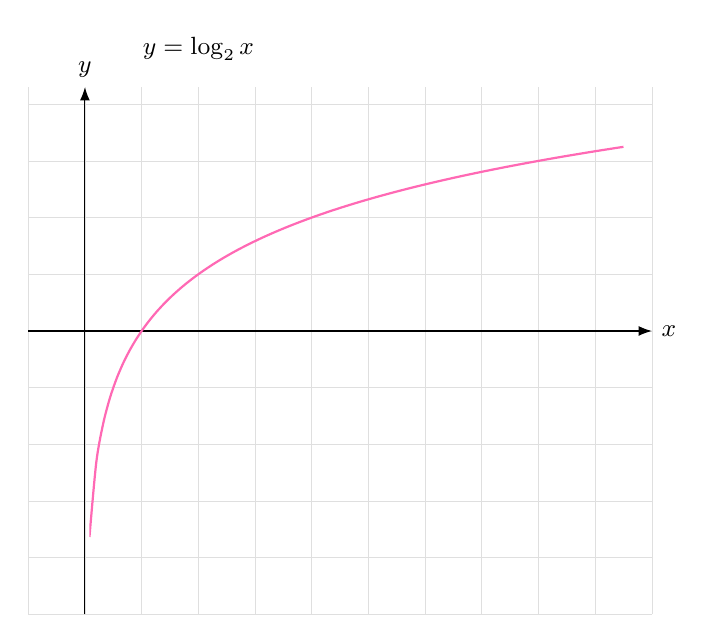
\begin{tikzpicture}[scale=0.72]
\begin{scope}
\node[above] at (2,4.6) {\small $y=\log_2 x$};
\draw[step=1, gray!25, very thin] (-1,-5) grid (10,4.3);
\draw[-{Latex}] (-1,0) -- (10,0) node[right] {\small $x$};
\draw[-{Latex}] (0,-5) -- (0,4.3) node[above] {\small $y$};
\begin{scope}
\clip (0.08,-5) rectangle (10,4.3);
\draw[pinkanno, thick, domain=0.08:9.5, samples=80, smooth] plot (\x, {ln(\x)/ln(2)});
\end{scope}
\end{scope}
\end{tikzpicture}
\end{center}

\textbf{Domain:} $(0,\infty)$. \quad \textbf{Range:} $(-\infty,\infty)$. \quad \textbf{Vertical Asymptote:} $x=0$.

\begin{center}
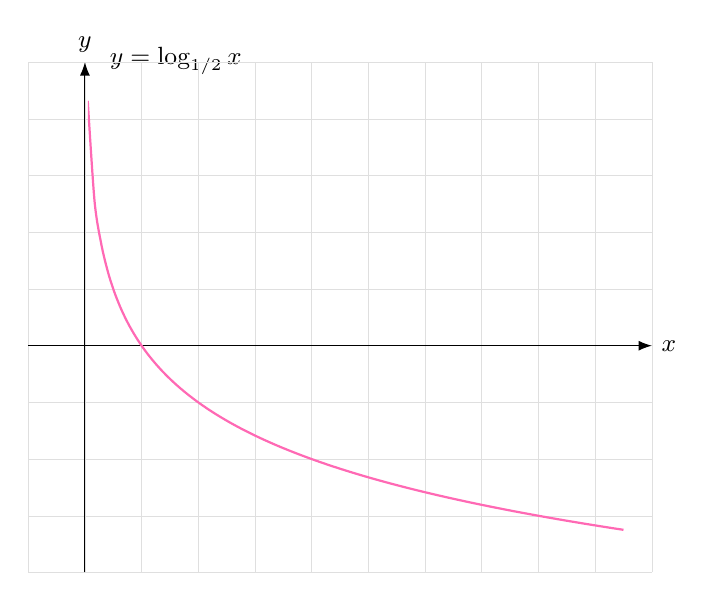
\begin{tikzpicture}[scale=0.72]
\node[above] at (1.6,4.6) {\small $y=\log_{1/2} x$};
\draw[step=1, gray!25, very thin] (-1,-4) grid (10,5);
\draw[-{Latex}] (-1,0) -- (10,0) node[right] {\small $x$};
\draw[-{Latex}] (0,-4) -- (0,5) node[above] {\small $y$};
\begin{scope}
\clip (0.05,-4) rectangle (10,5);
\draw[pinkanno, thick, domain=0.05:9.5, samples=80, smooth] plot (\x, {ln(\x)/ln(0.5)});
\end{scope}
\end{tikzpicture}
\end{center}

\textbf{Domain:} $(0,\infty)$. \quad \textbf{Range:} $(-\infty,\infty)$. \quad \textbf{Vertical Asymptote:} $x=0$.

\begin{friendlyrule}{Graph of $y=\log_a(x)$ in General}
\begin{itemize}
    \item \textbf{Domain:} $(0,\infty)$. \qquad \textbf{Range:} $(-\infty,\infty)$.
    \item \textbf{Vertical Asymptote:} $x=0$.
    \item \textbf{$x$-intercept:} $(1,0)$, since $\log_a(1)=0$ for any base $a$.
    \item \textbf{$y$-intercept:} none --- $x=0$ is not in the domain.
\end{itemize}
\end{friendlyrule}

\begin{center}
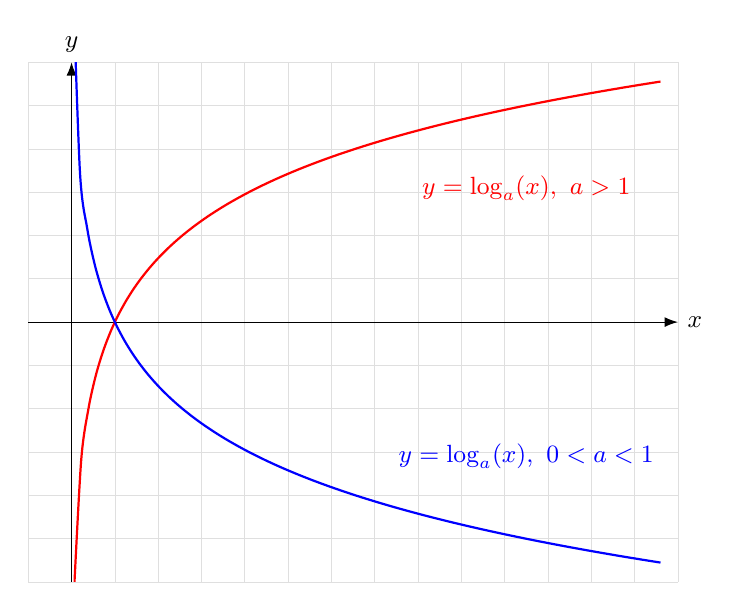
\begin{tikzpicture}[scale=0.55]
\draw[step=1, gray!25, very thin] (-1,-6) grid (14,6);
\draw[-{Latex}] (-1,0) -- (14,0) node[right] {\small $x$};
\draw[-{Latex}] (0,-6) -- (0,6) node[above] {\small $y$};
\begin{scope}
\clip (0.05,-6) rectangle (14,6);
\draw[red, thick, domain=0.05:13.6, samples=80, smooth] plot (\x, {ln(\x)/ln(1.6)});
\end{scope}
\node[red] at (10.5,3.1) {\small $y=\log_a(x),\ a>1$};
\begin{scope}
\clip (0.02,-6) rectangle (14,6);
\draw[blue, thick, domain=0.02:13.6, samples=80, smooth] plot (\x, {ln(\x)/ln(0.625)});
\end{scope}
\node[blue] at (10.5,-3.1) {\small $y=\log_a(x),\ 0<a<1$};
\end{tikzpicture}
\end{center}

\section*{3. Transformations of Logarithmic Graphs}

\begin{friendlyex}{}
Graph $f(x)=\log_2(x-3)+2$. Determine the domain, range, and vertical asymptote.
\end{friendlyex}

\begin{solutionbox}
This is $y=\log_2(x)$ shifted \textbf{$3$ units right} and \textbf{$2$ units up}.

\begin{center}
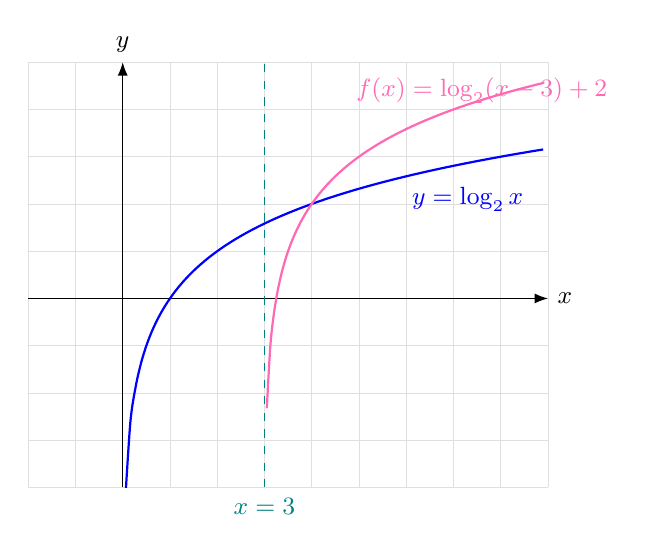
\begin{tikzpicture}[scale=0.6]
\draw[step=1, gray!25, very thin] (-2,-4) grid (9,5);
\draw[-{Latex}] (-2,0) -- (9,0) node[right] {\small $x$};
\draw[-{Latex}] (0,-4) -- (0,5) node[above] {\small $y$};
\draw[dashed, teal] (3,-4) -- (3,5);
\node[teal] at (3,-4.4) {\small $x=3$};
\begin{scope}
\clip (-2,-4) rectangle (9,5);
\draw[blue, thick, domain=0.05:8.9, samples=80, smooth] plot (\x, {ln(\x)/ln(2)});
\end{scope}
\node[blue] at (7.3,2.1) {\small $y=\log_2x$};
\begin{scope}
\clip (-2,-4) rectangle (9,5);
\draw[pinkanno, thick, domain=3.05:8.9, samples=80, smooth] plot (\x, {ln(\x-3)/ln(2)+2});
\end{scope}
\node[pinkanno] at (7.6,4.4) {\small $f(x)=\log_2(x-3)+2$};
\end{tikzpicture}
\end{center}

\textbf{Domain:} $x-3>0 \implies x>3$, i.e.\ $(3,\infty)$.

\textbf{Range:} $(-\infty,\infty)$ --- a vertical shift never restricts the range of a log function.

\textbf{Vertical Asymptote:} $x=3$.
\end{solutionbox}

\begin{friendlyex}{}
Determine the domain and vertical asymptote for the graph of $g(x)=\log(6-x)-3$.
\end{friendlyex}

\begin{solutionbox}
This is $y=\log(x)$ reflected about the $y$-axis, shifted right $6$, and down $3$.

\textbf{Domain:} we need $6-x>0 \implies x<6$, i.e.\ $\boxed{(-\infty,6)}$.

\textbf{Vertical Asymptote:} $6-x=0 \implies \boxed{x=6}$.
\end{solutionbox}

\section*{4. Applications}

\subsection*{The pH Scale}

\begin{friendlyrule}{pH Formula}
In chemistry, pH is defined by
\[
pH=-\log[H^+],
\]
where $[H^+]$ is the concentration of the hydrogen ion (in moles per liter).
\end{friendlyrule}

\begin{friendlyex}{}
Find the pH of the following.
\begin{enumerate}[label=(\alph*)]
    \item Lemon Juice, $H^+\approx 1.3\times 10^{-5}$
    \item Apples, $H^+\approx 2.7\times 10^{-6}$
\end{enumerate}
\end{friendlyex}

\begin{solutionbox}
\textbf{(a)}
\[
pH=-\log(1.3\times10^{-5})\approx \boxed{4.89}
\]

\textbf{(b)}
\[
pH=-\log(2.7\times10^{-6})\approx \boxed{5.57}
\]
\end{solutionbox}

\begin{friendlyex}{}
Find the $H^+$ concentration of the following.
\begin{enumerate}[label=(\alph*)]
    \item Soda Ash, with $pH=10.3$
    \item Bottled Water, with $pH=7$
\end{enumerate}
\end{friendlyex}

\begin{solutionbox}
Solve $pH=-\log[H^+]$ for $[H^+]$: \ $[H^+]=10^{-pH}$.

\textbf{(a)}
\[
[H^+]=10^{-10.3}\approx \boxed{5.01\times10^{-11} \text{ moles/liter}}
\]

\textbf{(b)}
\[
[H^+]=10^{-7} \text{ moles/liter}
\]
\end{solutionbox}

\subsection*{The Richter Scale}

\begin{friendlyrule}{Richter Scale Formula}
For an earthquake of intensity $I$, its magnitude $R$ on the Richter scale is
\[
R=\log\frac{I}{I_0},
\]
where $I_0$ is the reference intensity --- the smallest earth movement detectable on a seismograph. Each unit rise on the Richter scale corresponds to a $10$ times increase in intensity.
\end{friendlyrule}

\begin{friendlyex}{}
Find the magnitude of an earthquake whose intensity is
\begin{enumerate}[label=(\alph*)]
    \item $50{,}000\, I_0$
    \item $500{,}000\, I_0$
\end{enumerate}
\end{friendlyex}

\begin{solutionbox}
\textbf{(a)}
\[
R=\log\left(\frac{50000\,I_0}{I_0}\right)=\log(50000)\approx \boxed{4.70}
\]

\textbf{(b)}
\[
R=\log\left(\frac{500000\,I_0}{I_0}\right)=\log(500000)\approx \boxed{5.70}
\]
\end{solutionbox}

\begin{friendlyex}{}
How many times more intense is an earthquake with a magnitude of $6.7$ than one with a magnitude of $4.7$ on the Richter Scale?
\end{friendlyex}

\begin{solutionbox}
Each unit on the Richter scale is a factor of $10$ in intensity, so
\[
10^{6.7-4.7}=10^2=\boxed{100 \text{ times more intense}}
\]
\end{solutionbox}

\section*{Summary}

\begin{friendlyrule}{Key Ideas}
\begin{itemize}
    \item $y=a^x$ is equivalent to $x=\log_a(y)$; logarithmic and exponential functions are inverses of each other.
    \item Natural log: $\log_e x=\ln x$. \quad Common log: $\log_{10}x=\log x$.
    \item $\log_a(x)$ is only defined for $x>0$ --- the logarithm of zero or a negative number does not exist.
    \item The graph of $y=\log_a(x)$ has domain $(0,\infty)$, range $(-\infty,\infty)$, vertical asymptote $x=0$, and $x$-intercept $(1,0)$ (no $y$-intercept).
    \item Writing $f(x)=\log_a(x-h)+k$ shifts the graph $h$ units horizontally and $k$ units vertically, moving the vertical asymptote to $x=h$; the range always stays $(-\infty,\infty)$.
    \item Applications: pH $=-\log[H^+]$, and the Richter scale $R=\log(I/I_0)$, where each whole-number increase means $10\times$ the intensity.
\end{itemize}
\end{friendlyrule}

\end{document}
